\chapter{Calculate the electronic structure of a hydrogen molecule}\label{ch:first}

A hydrogen molecule has only two atoms, yet introduces the essentials of an electronic structure calculation: where to place the atoms, how the electrons are distributed, how to recognize completion, and which geometry the final numbers describe. Starting from a prepared file, this chapter runs a self-consistent field calculation and examines the energy and error histories. The same procedure can then be applied to larger molecules and crystals.

The example uses plane waves and pseudopotentials. You do not need their mathematical derivation for a first run. Learn the structures, nodes, and results in the interface first, then read Chapter~\ref{ch:theory} to understand the parameters in that practical context.

\section{Prepare the hydrogen example}

Two hydrogen atoms are placed in a cubic simulation box. Their positions remain fixed while the electronic ground state is calculated. This is a single-point energy calculation: ``single point'' means one geometry, not one numerical iteration. The density is updated repeatedly until successive solutions agree sufficiently well, a procedure called self-consistent field calculation, or SCF.

At the end, your project should contain a hydrogen structure, a reusable workflow, and an energy/error plot. Save it for the later geometry-optimization tutorial. For a first run, use the current workspace's computing environment; Online performs the same steps in its server session.

\begin{table}[htbp]
\centering
\caption{Calculation conditions for the hydrogen tutorial.}
\begin{tabularx}{\linewidth}{lX}
\toprule
Item & Setting\\
\midrule
Structure type & Molecule\\
Simulation box & Cube with sides of $10$ Bohr, approximately $5.29177$ Å\\
Hydrogen positions & Fractional coordinates $(0.5,0.5,0.425)$ and $(0.5,0.5,0.575)$\\
Initial bond length & $1.5$ Bohr, approximately $0.793766$ Å\\
Exchange-correlation functional & PBE\\
Pseudopotential & default, built-in PBE-1.3 ONCV pseudopotentials\\
Plane-wave cutoff & $20$ Ha\\
Spin components & Nspin = 1\\
Temperature & $0$ K\\
SCF method & davidson\_qe; maximum $100$ iterations\\
Forces & Calculate force selected\\
\bottomrule
\end{tabularx}
\end{table}

\file{examples/h2.cif} stores this box and these atomic positions. Using it avoids manual coordinate entry and gives desktop and Online sessions the same starting structure. Here, the CIF lattice describes the simulation box; you must still select \ui{Molecule} in the \ui{Build Molecule} node. File format and calculation-object type are separate choices.

\begin{notebox}{Why start with a small molecule?}
A small system makes every step easy to inspect and parameter changes easy to compare. The specified box and cutoff let you complete the exercise and compare results. Test their convergence again when using another molecule.
\end{notebox}

\section{Create a project and import the structure}

\subsection{Use a separate project}

A project holds the structure, workflow, and results together. Give it a clear name so that you can recognize its purpose when returning later. For example, call this one ``Hydrogen introduction'' and save it as \file{h2-first.ks}. The application starts with an empty project. If another project is open, save it and close it to return to an empty one.

\begin{steps}
\item If another project is open, save it and choose \ui{Home → Close}.
\item Check that the Project Browser shows categories for structures, workflows, and results.
\item Keep the empty project open and proceed with import.
\item After importing, use \ui{Save} to choose a project name and location.
\end{steps}

Desktop editions normally use a system file dialog for local files. Online file selection and downloads pass through the browser: supply the tutorial file to the session, then select it in the application. In either environment, the imported structure must appear in the Project Browser, not merely in the browser's download list.

\subsection{Import hydrogen}

\begin{steps}
\item On \ui{Home}, choose \ui{Import structure from file...} from Structure.
\item Select the supplied \file{h2.cif}.
\item Select the imported structure in the Project Browser, expand the \ui{Information Browser} below, and check the elements and atom count. If the panel is missing, select it from the ellipsis button's \ui{Open Panels} list.
\item Open the structure's 3D view and rotate it until both hydrogen atoms are clearly visible.
\end{steps}

You should see two hydrogen atoms. The box boundary may be visible or hidden according to display settings. Sphere sizes and bond styles affect only the picture, not atomic coordinates. Use fit-to-view or zoom if the structure is off-center or outside the view.

\subsection{Check the geometry}

Before calculating, measure the distance between the atoms in the viewer. The input bond length is approximately $0.793766$ Å. The displayed precision may differ; $0.794$ Å agrees with this input. The underlying numerical coordinate unit is Bohr, giving a bond length of $1.5$ Bohr.

You can also select a hydrogen atom to inspect its coordinate card. Figure~\ref{fig:h2-structure-inspection} selects site 2, with fractional coordinates $(0.500,0.500,0.575)$ and displayed Cartesian coordinates $(2.646,2.646,3.043)$ Å. Fractional coordinates locate the atom relative to the box; Cartesian coordinates give its position in Å. Both atoms lie near the box center with space around them. A CIF-imported document may show \ui{Crystal Modeling}; the solver must nevertheless use \ui{Molecule} in the structure configuration node for this example.

\begin{figure}[!htb]
\centering
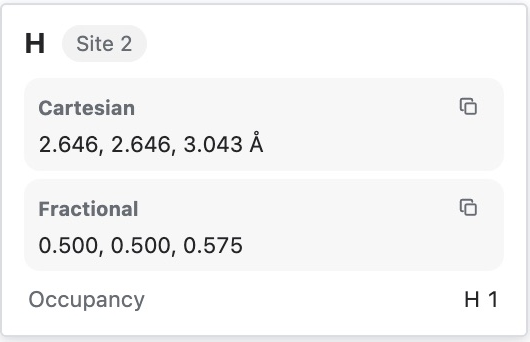
\includegraphics[width=79mm]{publication-assets/crop-f7556efd0d7de78b7cf1.png}
\caption{The coordinate card for site 2 of the initial hydrogen molecule, showing Cartesian coordinates, fractional coordinates, and occupancy. Use it to check the selected site's geometry.}
\label{fig:h2-structure-inspection}
\end{figure}

Electronic structure depends on atomic positions. For this exercise, confirm two hydrogen atoms, a bond length of approximately $0.794$ Å, and a cubic box of approximately $5.292$ Å per side.

An XYZ file can reproduce the same bond length without reproducing the same box. When a molecular file has no lattice, the software constructs a box from the atomic extent and vacuum spacing. Use an identical simulation box, as well as bond length, for a detailed numerical comparison with this chapter.

\section{Build the SCF workflow}

\subsection{Start with the \headinglatin{SCF} template}

A workflow divides the calculation into nodes, connected in processing order. This example needs three tasks: pass the imported structure to the solver, calculate the electronic structure, and display convergence. A template establishes these connections before you adjust individual settings.

\begin{steps}
\item Open the \ui{Workflow} import menu and choose \ui{Import workflow from template}.
\item Select the \ui{SCF} template.
\item Open the new workflow document and inspect its nodes and connections.
\item Check that structure configuration, SCF, and energy plotting are connected in that order. The structure node may be labeled \ui{Configuration} or \ui{Build Molecule}; both refer to the same task. The next nodes are \ui{SCF} and \ui{Plot}.
\end{steps}

With a blank workflow, add and connect these three nodes yourself. Display labels can be edited, but task types must remain correct. Renaming a node to ``Calculate hydrogen,'' for example, does not change its SCF task type. Keep template names for your first run so that they match the tutorial.

Use Figure~\ref{fig:h2-workflow} to check the sequence: the first node supplies the structure, the second solves its electronic structure, and the last plots the calculation history. Configure them in that order.

\begin{figure}[!htb]
\centering
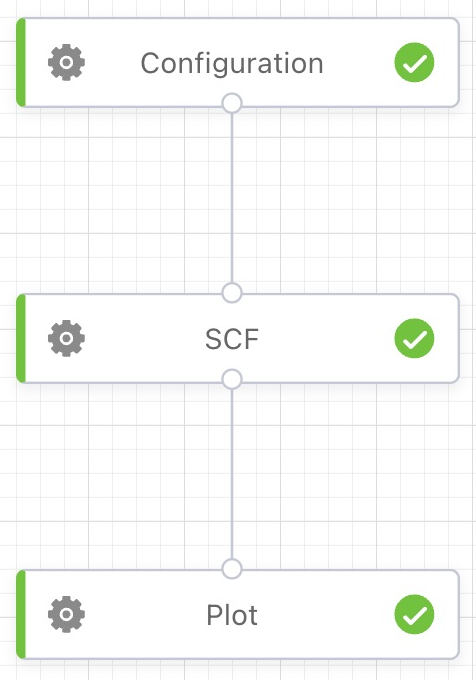
\includegraphics[width=60mm]{publication-assets/crop-273037e846506daab173.png}
\caption{The hydrogen SCF workflow. Structure configuration, electronic solving, and plotting run from top to bottom. Configuration is the Build Molecule task, and Plot produces the convergence curve.}
\label{fig:h2-workflow}
\end{figure}

\subsection{Configure structure input}

Select \ui{Configuration}, then choose \ui{Workflow → Configure Node} or click its gear. This opens the right-side panel if collapsed and opens or refreshes the task settings in the \ui{Config Editor}. Scroll to \ui{Options} to find Type and the other parameters. If only general properties such as ID, label, and module are visible, invoke Configure Node first. This node selects the structure and defines the physical and numerical model. Check each input before running.

A narrow panel may truncate parameter labels or dropdown values. Open the ellipsis at the upper right of the \ui{Config Editor} title bar and choose \ui{Maximize} to give it more space. Use \ui{Restore} in the same menu afterward to return to the side-by-side layout. \ui{General}, \ui{Inputs}, \ui{Options}, and \ui{Advanced Options} expand independently. Collapse General and Inputs while entering the tutorial settings if needed.

\begin{steps}
\item Set \ui{Type} to \ui{Molecule}.
\item Under \ui{Choose imported structures}, select only this hydrogen structure.
\item Set \ui{Functional} to \ui{PBE} and \ui{Pseudopotential} to \ui{default}.
\item Enter \texttt{20} in \ui{Ecut (Hartree)}.
\item Keep \ui{Smearing} at \ui{fermi-dirac}, \ui{Temperature (K)} at \texttt{0}, and \ui{Nspin} at \texttt{1}.
\item In Advanced Options, keep Extra bands at \texttt{0}.
\end{steps}

With Molecule selected, automatic crystal $k$-point settings are not part of this exercise. The molecule-in-a-box calculation does not need a crystal sampling grid.

Pay particular attention to \ui{Ecut (Hartree)}. Entering $20$ means $20$ Ha, approximately $544$ eV, not $20$ eV. The interface gives the unit in the label. Convert units before comparing parameters with papers or other software.

\begin{figure}[H]
\centering
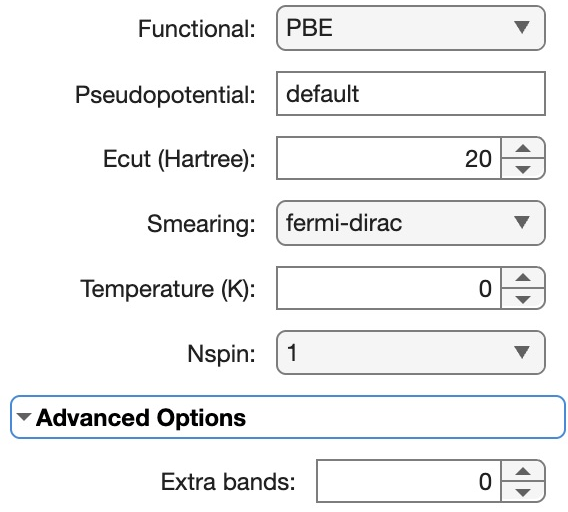
\includegraphics[width=90mm]{publication-assets/crop-1d148adc90da2955994e.png}
\caption{Regular and advanced structure-node options. Check PBE, default pseudopotentials, 20 Ha, 0 K, Nspin=1, and Extra bands=0 here. Figure~\ref{fig:online-h2-config} shows the Molecule and h2 selections.}
\label{fig:h2-build-options}
\end{figure}

\subsection{Configure \headinglatin{SCF}}

Select \ui{SCF}, choose \ui{Workflow → Configure Node}, and scroll to \ui{Options}. \ui{DiagMethod} selects the numerical method for solving electronic states at each iteration; \ui{Max SCF steps} limits density updates. Use the default \ui{davidson\_qe} and $100$ iterations here.

The \ui{DiagMethod} dropdown offers several methods. Choose \ui{davidson\_qe}; if the closed field truncates it, maximize the panel to check the complete name.

\begin{figure}[!htb]
\centering
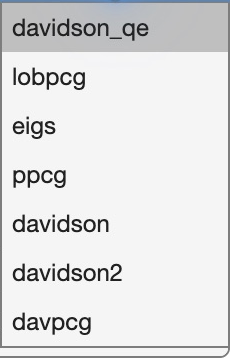
\includegraphics[width=48mm]{publication-assets/crop-1581def0867bec552a40.png}
\caption{The SCF algorithm list, with davidson\_qe selected for this example.}
\label{fig:h2-scf-methods}
\end{figure}

Select \ui{Calculate force}. Atomic forces indicate directions in which moving atoms would locally lower the energy for the current electronic state. This chapter holds positions fixed; calculating forces lets you compare the starting and optimized structures later. An ordinary single-point energy calculation can leave this option cleared when forces are not needed.

Keep the advanced \ui{ExxMethod} at \ui{default}. It mainly concerns hybrid-functional calculations and needs no adjustment for this PBE example.

Use Table~\ref{tab:h2-scf-options} for a final check. Maximize the Config Editor to read long method names, then restore the layout.

\begin{table}[!htb]
\centering
\caption{SCF settings for the hydrogen tutorial.}
\label{tab:h2-scf-options}
\begin{tabularx}{\linewidth}{lX}
\toprule
Option & Setting\\
\midrule
\ui{DiagMethod} & \ui{davidson\_qe}, the electronic-state solver at each iteration\\
\ui{Max SCF steps} & \texttt{100}, the maximum density updates\\
\ui{Calculate force} & Selected to calculate forces in this single-point run\\
\ui{ExxMethod} & \ui{default}, retaining the advanced default\\
\bottomrule
\end{tabularx}
\end{table}

\subsection{Check the plotting node}

The energy-curve task, labeled \ui{Plot} here, draws the SCF history. It does not solve the electronic structure again or alter the preceding result. Check that it follows SCF. If you add it after an SCF run, rerun this complete small workflow to obtain a plot tied to that run.

Save before running. The saved workflow records the conditions directly when you later compare cutoffs, structures, or functionals.

\section{Run the calculation and follow progress}

\subsection{Activate the intended workflow}

Several workflow documents can be open at once. Select this workflow's document tab before choosing \ui{Run}, so that a different workflow is not executed accidentally.

Expand the right panel group and the \ui{Simulation Browser} title bar. Reopen it by name from \ui{Open Panels} if closed. If configuration still fills the workspace, use \ui{Restore} in its title menu to view the canvas and output together. The browser displays messages as the calculation starts. SCF output normally lists error, total energy, and time by iteration. A slowly decreasing error at one step need not indicate a mistake. Judge the full history and final convergence status.

\begin{steps}
\item Activate the hydrogen SCF workflow document.
\item Choose \ui{Home → Run}, or use \ui{Run} in the Simulation Browser.
\item Find the message marking the start of the hydrogen calculation.
\item Wait for convergence, then inspect the plot that opens automatically.
\item Return to the canvas and check that all required nodes finished.
\end{steps}

The local \ui{Stop} button resets the run-button state but does not interrupt an ongoing numerical solve. Synchronous Online calculations also offer no stop operation. Wait for this example to finish. Read the log for progress; closing a browser tab neither saves the project nor ends the server calculation.

\subsection{Measure elapsed time}

The dropdown next to \ui{Run} offers \ui{Run and time}. Activate this SCF workflow and choose it. When a local run finishes, the window bottom reports its elapsed time. This includes execution and associated preparation for the whole workflow, not a separate performance profile for each node.

Compare timings only with the same model, settings, and execution environment, and state whether a run was the first one. Initializing numerical functions or creating a figure can add startup time. For a remote submission, local submission time is not remote calculation time; read the remote job records. Record timing separately in your notes if useful. Scientific validity still rests on energy, error, and convergence.

\subsection{Read the three main log values}

Begin with iteration number, relative density error, and total energy. The iteration number counts updates, density error measures the difference between successive input and output densities, and total energy estimates the system's energy at the current density.

Energy generally stabilizes as density becomes self-consistent, but need not decrease monotonically. Mixing historical densities can cause a temporary increase during an otherwise normal iteration sequence. Read the final convergence message rather than judging completion from two nearly equal energy entries.

\begin{figure}[!htb]
\centering
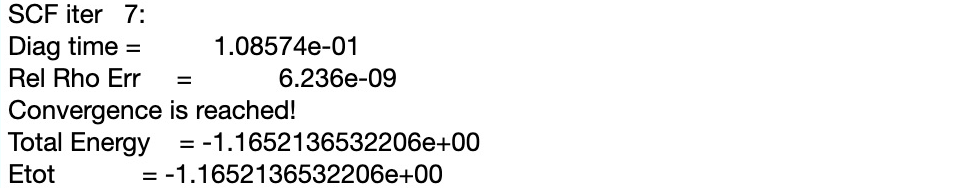
\includegraphics[width=119.9mm]{publication-assets/crop-2984400ea30d3f4eb1f5.png}
\caption{Part of the hydrogen SCF log. Iteration 7 reports \ui{Convergence is reached!}, with total energy $-1.1652136532206$ Ha and relative density error approximately $6.24\times10^{-9}$.}
\label{fig:h2-scf-runtime-log}
\end{figure}

\section{Read your first calculation result}

\subsection{Understand the convergence plot}

The plot combines two histories from the same SCF run. Iteration number is horizontal, total energy in Ha uses the left axis, and error uses the right. The logarithmic error axis means that equal vertical distances can correspond to one or more orders of magnitude.

Read the energy from left to right, then check whether the error decreases overall. In this small hydrogen molecule, energy is nearly stable after the first few iterations while the density error still needs to fall. A visually flat curve and a satisfied convergence criterion are different things.

\begin{figure}[!htb]
\centering
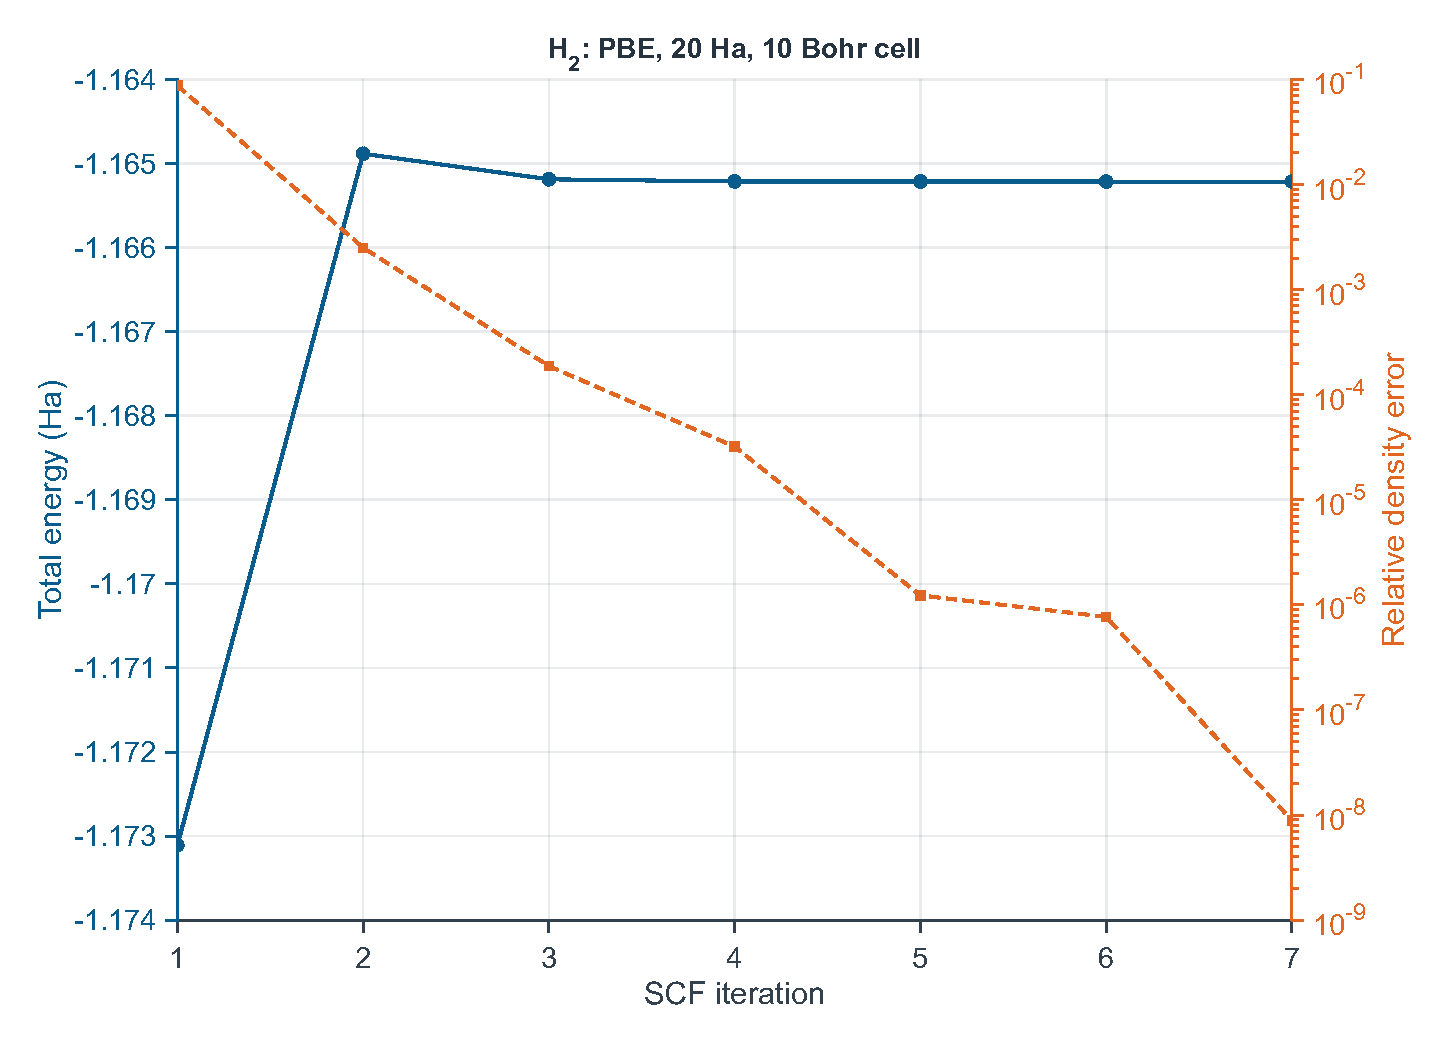
\includegraphics[width=\linewidth]{publication-assets/vector-2e572f3c8654292658e8.pdf}
\caption{Total energy and relative density error for hydrogen SCF. Read the blue line against the left axis and the orange dashed line against the logarithmic right axis. Data are from the supplied reference run.}
\label{fig:h2-scf-results}
\end{figure}

\subsection{Compare with the reference run}

The accompanying script converges in $7$ iterations, with total energy approximately $-1.1652136531$ Ha and final relative density error approximately $8.85\times10^{-9}$. Use these values to compare your result.

The run in Figure~\ref{fig:h2-scf-runtime-log} also converges in 7 iterations, at approximately $-1.1652136532$ Ha and $6.24\times10^{-9}$ relative density error. Both meet the example's convergence criterion. Figure~\ref{fig:h2-scf-results} plots the history saved by the script.

Initial electronic states, software versions, and numerical environments may change iteration counts or the final digits in a graphical run. First match the structure, box, functional, pseudopotentials, and cutoff, then check convergence. Timing also depends on hardware and session load. Use the numerical results and convergence state to assess agreement.

\begin{notebox}{What this total energy means}
This energy belongs to hydrogen at this geometry, in this box, with this functional and pseudopotentials. It is not directly an experimental binding energy. A dissociation-energy calculation also needs consistently calculated atomic reference states, including appropriate spin treatment.
\end{notebox}

\subsection{Save results and the project}

Once added under Results, the plot can be reopened from the Project Browser. A figure presents the calculation record; the workflow records how it was obtained. Keep both. Save the project after the run as well as before it.

Use a clear figure name such as ``Hydrogen: PBE, 20 Ha, initial geometry.'' Distinct names prevent confusion with later optimized-geometry results. Include the main conditions in the name and retain complete parameters in the workflow rather than creating an excessively long filename.

\section{Complete the exercise}

Reopen the saved project and check that the structure, workflow structure selection, and plot are restored.

For an extension, import \file{h2.cif} again and name it \file{H2-longer}. Use the geometry-editing procedure in Chapter~\ref{ch:modeling} to set a bond length of $0.85\,\text{\AA}$. Return to \ui{Build Molecule}, select this structure under \ui{Choose imported structures}, and run another single-point calculation without changing cutoff, functional, or box. Save both results and compare total energy and force along the bond. Chapter~\ref{ch:workflows} continues with geometry optimization; Chapter~\ref{ch:results} explains result interpretation.

\section{Reproduce the example with a script}

This section is for full MATLAB\regmark{} users. Standalone and Online users can continue with the graphical procedures without running the script. The interface is useful for learning and inspecting structures; scripts make repeated identical settings convenient. \file{examples/h2_scf_and_relax.m} contains the complete input. The excerpt below is its single-point calculation and assumes an initialized KSSOLV numerical environment.

\Needspace{11\baselineskip}
\begin{lstlisting}[language=Matlab]
pseudopotential.PpType('default');
molecule = example.structure.H2();
molecule.ecut = 20;
molecule.funct = 'PBE';
scfOptions = options.SCF('force', true);
scfOptions.enableGPU = false;
scfOptions.enableParallelPool = false;
[molecule, H, X, info] = scf(molecule, scfOptions);
\end{lstlisting}

In the returned values, \texttt{info.Etot} is the total energy, \texttt{info.Etotvec} and \texttt{info.SCFerrvec} hold the energy and error histories, and \texttt{info.converge} gives convergence status. Use them for tables or plots. The full script also optimizes positions and saves data. Run only the single-point section above to reproduce this chapter. The interface and script use the same numerical model; retain the explicitly specified tutorial parameters.
